%%%%%%%%%%%%%%%%%%%%%%%%%%%%%%%%%%%%%%%%%%%%%%%%%%%%%%%%%%%%%%%%%%%%%%%%
%% Description: Slides propostos para ANOVA - Aula 01 - Analise de
%% Variancia - parte I...
%% 
%% Maintainer: Rodrigo Sant'Ana - UNIVALI/GEP - Curso de Eng. Ambiental
%% e Sanitária e Eng. Ambiental
%% Author: Rodrigo Sant'Ana
%% Created: Seg Mar  9 21:08:55 2015 (-0300)
%% Version: 0.0.1
%% Last-Updated: Ter Mar 10 22:37:01 2015 (-0300)
%%           By: Rodrigo Sant'Ana
%% 
%% URL: http://github.com/rodrigosantana/Estatistica_II_EAS_EA_2015-1
%% Doc URL: http://github.com/rodrigosantana/Estatistica_II_EAS_EA_2015-1
%% 
%% Database info: 
%% 
%%% Commentary: 
%% 
%%% Code:
%%%%%%%%%%%%%%%%%%%%%%%%%%%%%%%%%%%%%%%%%%%%%%%%%%%%%%%%%%%%%%%%%%%%%%%%

\documentclass{bredelebeamer}

%%%%%%%%%%%%%%%%%%%%%%%%%%%%%%%%%%%%%%%%%%%%%%%%%%%%%%%%%%%%%%%%%%%%%%%%
%%% Configuracao da apresentacao...

%%% Titulo da apresentacao
\title[Análise de Variância]{Análise de Variância - Parte I}

%%% Subtitulo da apresentacao, se for necessario
%\subtitle{}

%%% Autor da apresentacao ou trabalho... \inst{num} corresponde ao link
%%% a instituicao que o autor esta vinculado
\author{Rodrigo Sant'Ana\inst{1}}

\institute[Universidade do Vale do Itajaí]
{
  \inst{1}%
  Universidade do Vale do Itajaí - UNIVALI\\
  Centro de Ciências Tecnológicas, da Terra e do Mar - CTTMar\\
  Curso de Engenharia Ambiental e Sanitária - EAS\\
  Curso de Engenharia Ambiental - EA\\
  Laboratório do Grupo de Estudos Pesqueiros - GEP
  }

%%% Periodo do curso...
\date{\footnotesize{Março, 2015}}

%%% Nao faco ideia onde este comando esta atuando...
\subject{}

\logo{

\includegraphics[scale=0.08]{images/univali.jpg}
}

%%%%%%%%%%%%%%%%%%%%%%%%%%%%%%%%%%%%%%%%%%%%%%%%%%%%%%%%%%%%%%%%%%%%%%%%
%%% Inicio do documento...
\begin{document}

%%% Slide de abertura...
\begin{frame}
  \titlepage
\end{frame}

%%% Slide de summario...
\begin{frame}{Sumário}
  \tableofcontents
\end{frame}

%%% Slide de conteudo - Secao 01...
\section{Concepção Geral}

\subsection{Definição}

\begin{frame}{Análise de Variância}
\begin{block}{Análise de Variância - ANOVA}
Trata-se de um método estatístico que permite realizar comparações
simultâneas entre três ou mais médias, ou seja, permite testas
\emphblue{hipóteses} sobre médias de diferentes populações.
\end{block}

\pause\begin{alertblock}{Importante}
Na ANOVA o termo \emph{Variância} se refere ao método utilizado e
\emph{não} à estatística que está sendo testada. \\
\vspace{.5cm}
\begin{flushright}
\emph{Estamos testando médias...}
\end{flushright}
\end{alertblock}
\end{frame}

\subsection{Ideia básica}

\begin{frame}
\begin{exampleblock}{Ideia básica}
A Análise de Variância (ANOVA) se estrutura no particionamento da
variabilidade contrariando o próprio nome. Neste sentido, este método
\underline{não} está preocupado em analisar \exemple{variância}, mas
\underline{sim}, a variabilidade nas médias ou no em torno delas. 
\end{exampleblock}

\begin{columns}
\begin{column}{0.5\textwidth}
\begin{center}
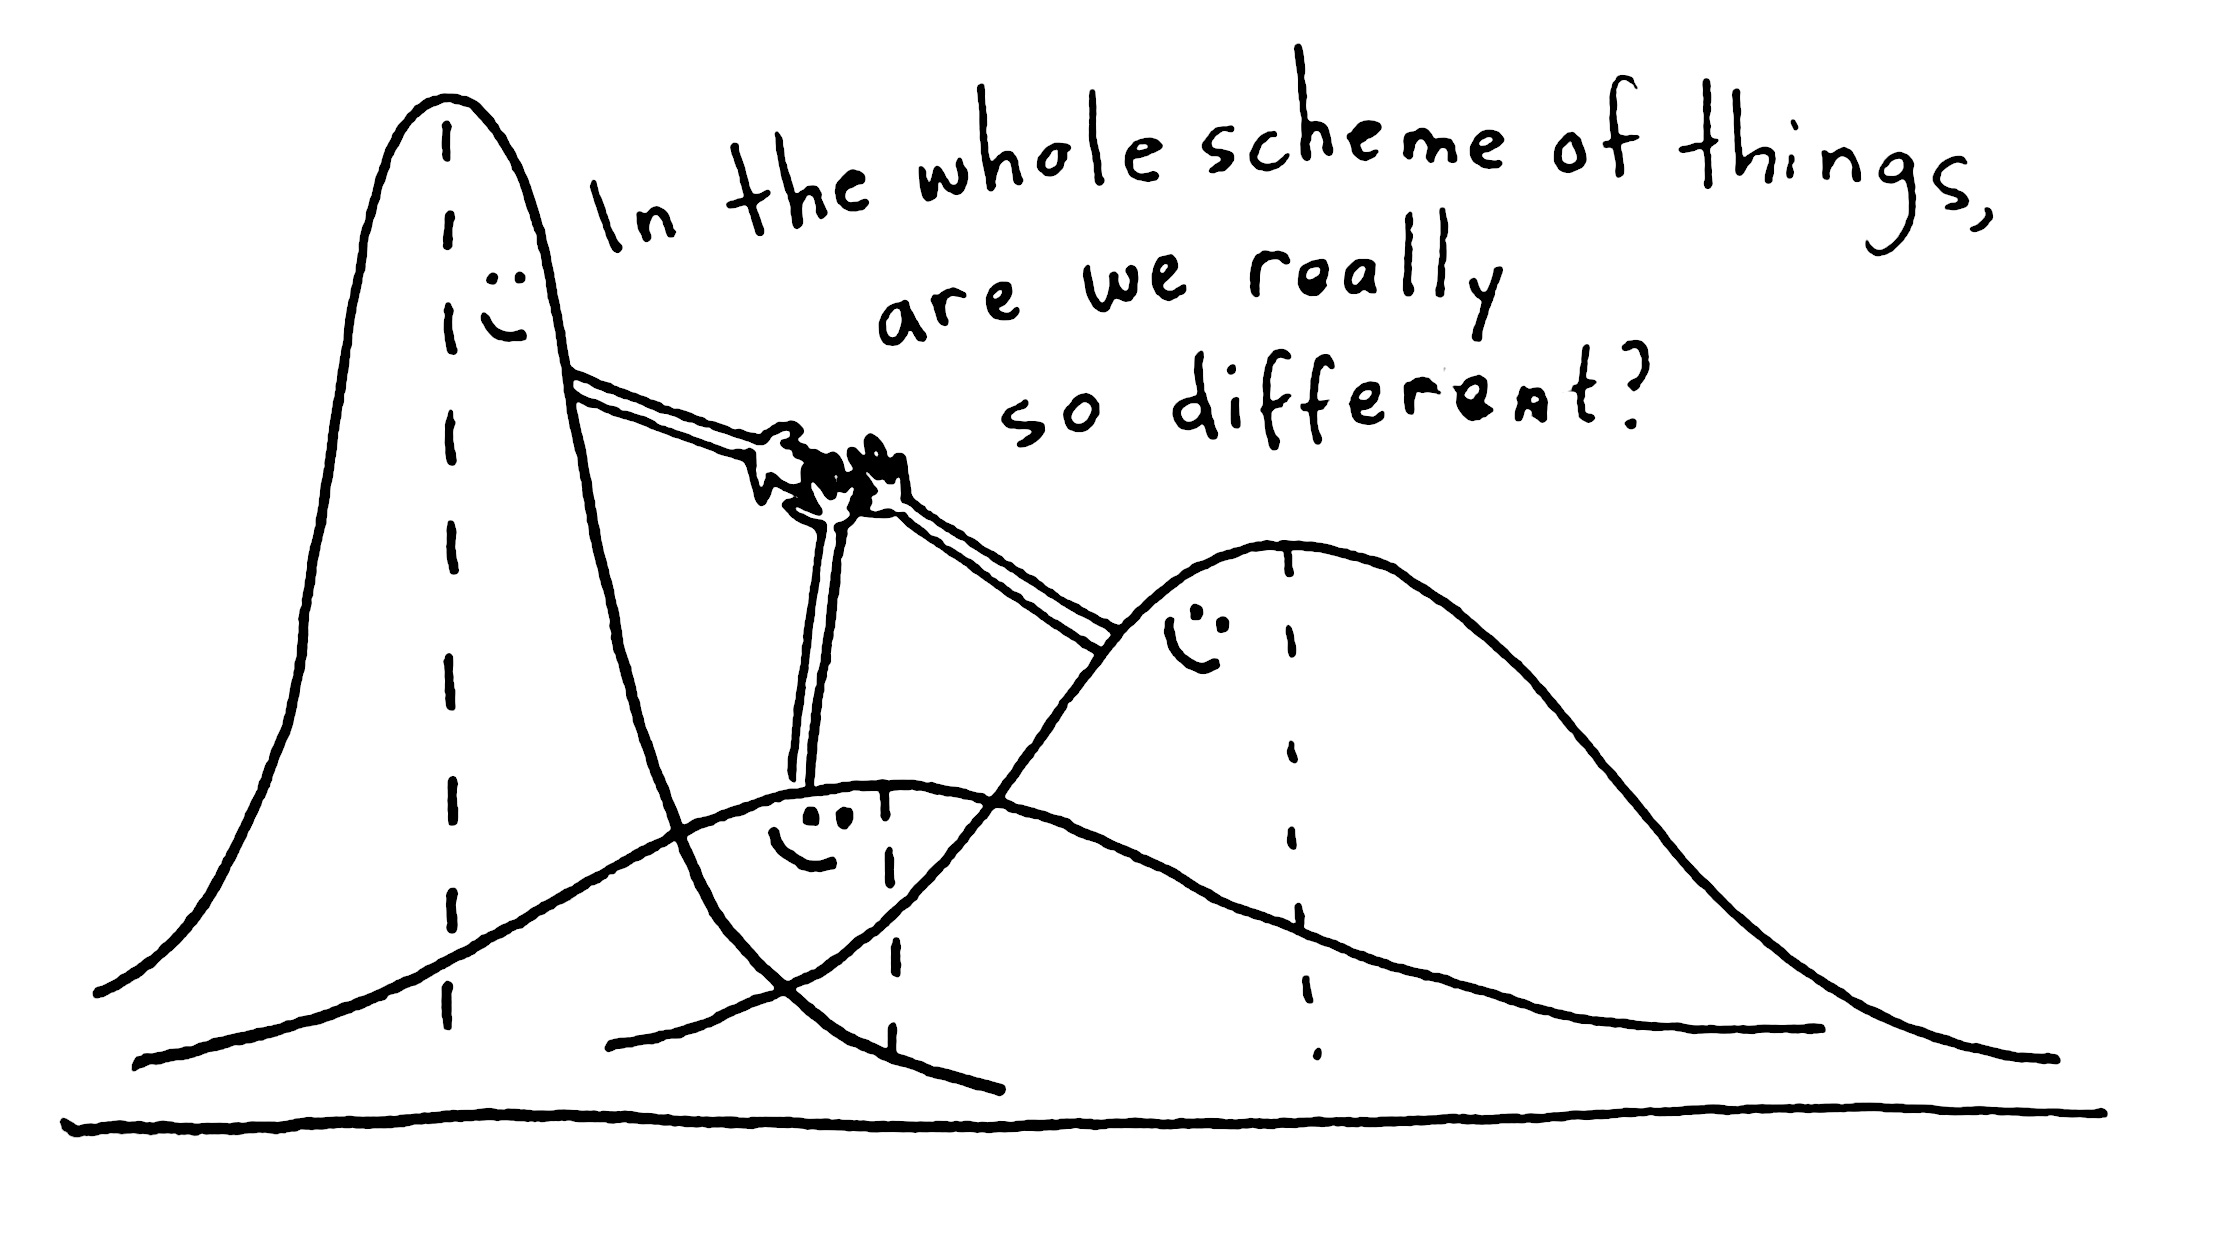
\includegraphics[scale=0.08]{images/anova.jpg}
\end{center}
\end{column}

\begin{column}{0.5\textwidth}
\begin{itemize}
\item $H_{0}: \mu_{1} = \mu_{2} = ...  = \mu_{k}$ \\
\item $H_{1}$\small{: pelo menos uma média é distinta das demais.}
\end{itemize}
\end{column}
\end{columns}
\end{frame}

\subsection{Pergunta universal}

\begin{frame}
\centering\textbf{\textcolor{red}{Por que aprender um novo método chamado
    ANOVA, quando simplesmente poderíamos conduzir uma série de testes 
    $T$ encadeados??}} 

\vspace{.6cm}

\pause
\begin{columns}
\begin{column}{.5\textwidth}
\begin{center}
\boitejaune{
\centering\textbf{\textcolor{Green}{ANOVA}}
}
\vspace{.5cm}
$\mu_{1} = \mu_{2} = \mu_{3}$ \\
\vspace{.5cm}
\small{\textbf{\exemple{Um único}} teste com $95\%$ de confiança \\
\vspace{.2cm}
ou seja, \\
\vspace{.2cm}
nível de significância $\alpha = 0.05$ \\
\vspace{.3cm}
\boiteblack{
\centering
(\% Confiança)$^{c}$ \hspace{.05cm} | \hspace{.05cm} 
$1 - (1 - \alpha)^{c}$}
}
\vspace{.3cm}
\centering\textcolor{Green}{``Boa ideia''}
\end{center}
\end{column}

\vline

\begin{column}{.5\textwidth}
\begin{center}
\boitegreen{
\centering\textbf{\textcolor{Framajaunelight}{Teste $T$}}
}
\vspace{.5cm}
$\mu_{1} = \mu_{2}$, $\mu_{1} = \mu_{3}$ e $\mu_{2} = \mu_{3}$ \\
\vspace{.5cm}
\small{\textbf{\alert{Três}} testes, cada um com $95\%$ de confiança \\
\vspace{.2cm}
ou seja, \\
\vspace{.2cm}
cada teste com um $\alpha = 0.05$ \\
\vspace{.3cm}
\boiteblack{
\centering
(\% Confiança)$^{c}$ \hspace{.05cm} | \hspace{.05cm} 
$1 - (1 - \alpha)^{c}$}
}
\vspace{.3cm}
\centering\textcolor{Red}{``Péssima ideia''}
\end{center}
\end{column}
\end{columns}
\end{frame}

\subsection{Erros de decisão}

\begin{frame}
\begin{center}
Quando mais de um teste $T$ é ajustado de forma encadeada, cada um com
seu respectivo nível de significância, a probabilidade de termos um erro
sobre a decisão é aumentada exponencialmente (\emph{Erro do Tipo I}).
\end{center}

\vspace{.1cm}

\begin{table}
\begin{tabular}{| >{\centering}m{0.8in} | >{\centering}m{0.8in} |
    >{\centering}m{1in} | >{\centering\arraybackslash}m{0.8in} |}
\hline
\rowcolor{Blue!60}
\multicolumn{4}{|r|}{Decisão} \\ \hline 
 & & \cellcolor{LightCyan}{Falha em rejeitar $H_{0}$} & 
 \cellcolor{Blue!20}{rejeita $H_{0}$} \\ \hline 
\multirow{2}{*}{
  \begin{sideways}
    Verdade
  \end{sideways}
}
 & $H_{0}$ é verdadeira & OK & \emph{Erro do Tipo I} \\[2ex] \cline{2-4}
 & $H_{1}$ é verdadeira & \emph{Erro do Tipo II} & OK \\[2ex] \hline
\end{tabular}
\end{table}

\vspace{.1cm}

\begin{flushright}
\textit{``We (almost) never know if $H_{0}$ ou $H_{1}$ is true, but we need to
  consider all possibilities''} \\
\footnotesize{Dr. Mine Çetinkaya-Rundel \\
Duke University}
\end{flushright}
\end{frame}

\subsection{Solução utilizada pelo método}

\begin{frame}
\begin{block}{Particionamento da variabilidade}
\centering
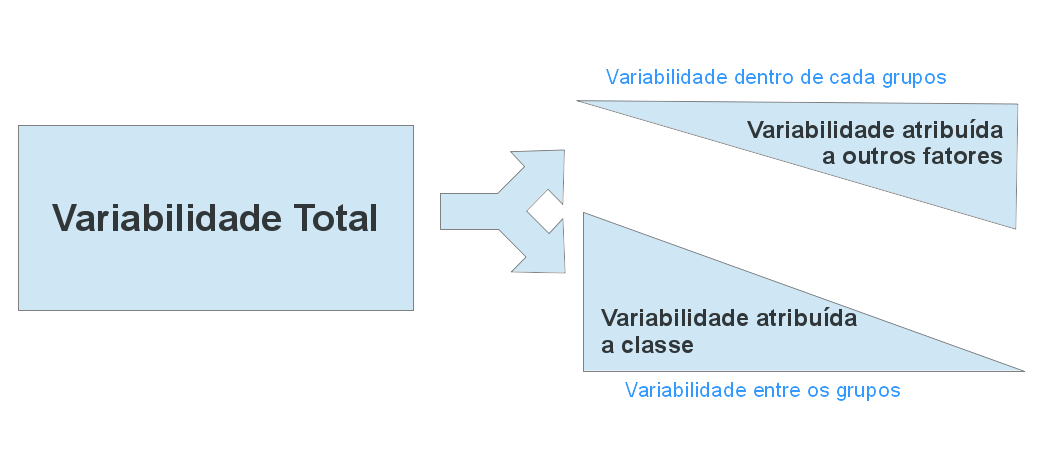
\includegraphics[scale=.4]{images/particionamento.png}
\end{block}
\end{frame}

\section{Pressupostos}

\begin{frame}
\begin{alertblock}{Pressupostos do método}
\begin{itemize}
\item[I)] Todas as observações devem ser independentes uma das outras e
  devem ser selecionadas aleatoriamente da população que representam;
\vspace{.5cm}
\item[II)] As populações de onde foram retiradas as amostras devem ter
  distribuições aproximadamente normais;
\vspace{.5cm}
\item[III)] As variâncias devem ser aproximadamente as mesmas entre as
  diferentes populações (homocedasticidade das variâncias).
\end{itemize}
\end{alertblock}
\end{frame}

\subsection{Independência das observações}

\begin{frame}
\begin{block}{Independência - considerações sobre o experimento}
Consiste em pressupor que os erros são \textit{variáveis aleatórias
  independentes}. Mas o que significa isto???
\end{block}

\pause
\vspace{.5cm}

Consideremos um experimento com voluntários... \\

\vspace{.5cm}

\begin{columns}
\begin{column}{0.5\textwidth}
\centering

\includegraphics[scale=1]{images/independencia.jpg}
\begin{center}
É razoável assumir ``Independência''
\end{center}
\end{column}

\begin{column}{0.5\textwidth}
\centering

\includegraphics[scale=.22]{images/dependente.jpg}
\begin{center}
É razoável assumir ``Dependência''
\end{center}
\end{column}
\end{columns}
\end{frame}

\begin{frame}
\begin{block}{Independência - análise de resíduos}
A análise gráfica dos resíduos é extremamente útil, porém não pode
associar um nível de probabilidade à conclusão de que os erros não são
independentes.
\end{block}

\vspace{.2cm}

\begin{columns}
\begin{column}{0.5\textwidth}
\centering
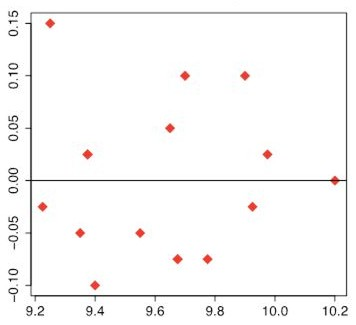
\includegraphics[scale=.22]{images/plot_indep.jpg}
\begin{center}
É razoável assumir ``Independência''
\end{center}
\end{column}

\begin{column}{0.5\textwidth}
\centering
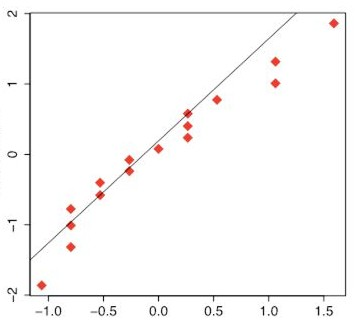
\includegraphics[scale=.22]{images/plot_dep.jpg}
\begin{center}
É razoável assumir ``Dependência''
\end{center}
\end{column}
\end{columns}


\vspace{.2cm}

\begin{flushright}
\footnotesize{
\textcolor{blue!75}{``Variáveis ou dados coletados em sequência - no
  tempo ou no espaço - geralmente têm correlação. Em outras palavras,
  medidas feitas na mesma unidade ou em unidades agrupadas, estão, muito
  frequentemente, correlacionadas''}} \\
\tiny{Sonia Vieira, \textit{Análise de Variância (ANOVA)}}
\end{flushright}
\end{frame}

\subsection{Homocedasticidade das variâncias}

\begin{frame}
\begin{alertblock}{Igualdade das variâncias}
\begin{columns}
\begin{column}{.5\textwidth}
\centering
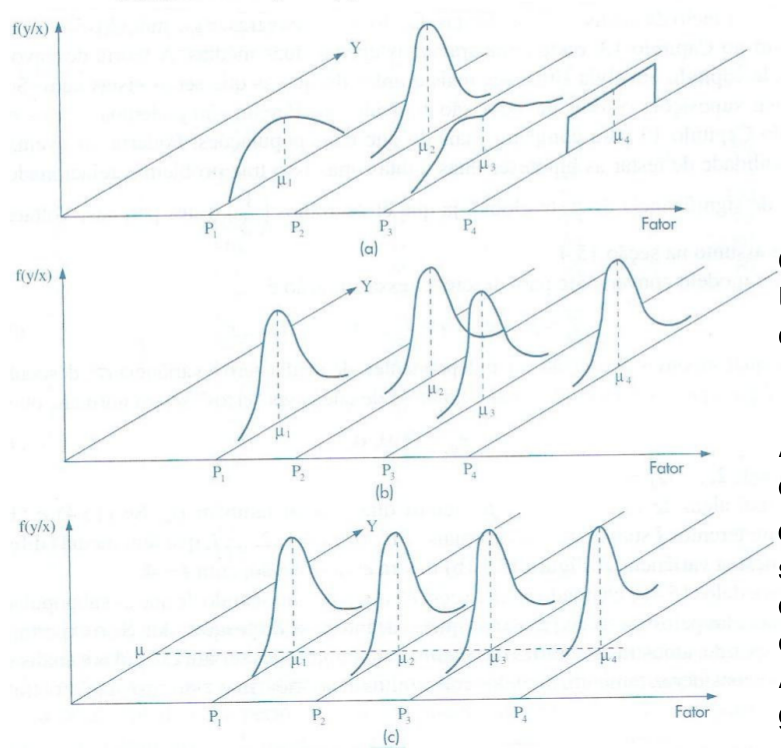
\includegraphics[scale=.18]{images/variancia.png}
\end{column}

\begin{column}{.45\textwidth}
\begin{center}
\footnotesize{
Regra prática - ``Cuidado ao usar!!!''
\begin{itemize}
\item Maior variância não exceda em três vezes a menor (Dean \& Voss,
  1999);
\item Maior variância não exceda em quatro vezes a menor (Box, 2000).
\end{itemize}
}

\vspace{.1cm}

\pause
\footnotesize{
Alternativa, testar igualdade de variâncias - ``Embora nenhum deles
tenha ampla recomendação!!!''
\begin{itemize}
\item teste de Cochran;
\item teste de Hartley;
\item teste de Bartlett;
\item teste de Levene.
\end{itemize}
}
\end{center}
\end{column}
\end{columns}
\end{alertblock}
\end{frame}

\begin{frame}
\begin{alertblock}{Variáveis obtidas por processos de contagem}
Em geral, variáveis discretas não possuem variância constante, muito
menos, distribuição aproximadamente normal. No entanto são utilizadas
comumente em análises de variância.

\vspace{.5cm}

Para estes casos, recomenda-se extrair a \emph{raiz quadrada}, assim,
esta nova variável (variável transformada), em geral, terá variância
constante.

\vspace{.5cm}

Este tipo de transformação é bastante eficaz pois reduz a
heterocedasticidade das variâncias.
\end{alertblock}
\end{frame}

\subsection{Distribuição (aproximadamente) normal}

\begin{frame}
\begin{exampleblock}{Normalidade}
\footnotesize{
Em geral, apesar de um pressuposto, este é o que menos impacta a análise
de variância como um todo. A menos que, a distribuição dos erros
(análise dos resíduos) mostre uma curtose positiva e assimetria.

\vspace{.2cm}

Nestes casos, as transgressões à pressuposição de normalidade irão
afetar o nível de significância do teste. 

\vspace{.2cm}

Em outras palavras, o pesquisador/analista de dados pensa que o nível de
significância ($\alpha$) do teste é 0,05 ou 5\%, mas na realidade está
trabalhando com um nível de significância de 7\% ou 8\%. 

\vspace{.2cm}

De todo modo, o teste $F$ é bastante robusto, pequenas transgressões à
pressuposição de normalidade são usuais e não afetam substancialmente os
resultados da análise. No entanto, a hipótese de normalidade dos erros
pode ser testada:

\begin{itemize}
\item teste $\chi^{2}$;
\item teste de Kolmogorov-Smirnov;
\item teste de Shapiro-Wilks.
\end{itemize}

}
\end{exampleblock}
\end{frame}

\section{Análise de Variância Simples}

\subsection{Modelo simples}

\begin{frame}
\begin{block}{ANOVA com um fator}
Suponhamos que estamos interessados em uma variável $Y_{ij}$, e que
poderíamos classificar os dados de acordo com uma característica $i$.

\vspace{.2cm}

Em uma ANOVA simples, estes dados são observados por um modelo linear
simples: 

\vspace{.2cm}

\begin{center}
$Y_{ij} = \mu_{i} + \epsilon_{ij}$, \hspace{.2cm} $i = 1, ..., k$ 
\hspace{.1cm} e \hspace{.1cm} $j = 1, ..., n$
\end{center}

\vspace{.2cm}

\begin{columns}
\begin{column}{.5\textwidth}
\centering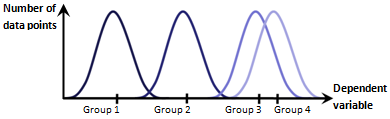
\includegraphics[scale=.3]{images/anova_distributions.png}
\end{column}

\begin{column}{.5\textwidth}
\begin{itemize}
\item $H_{0}$: $\mu_{1} = \mu_{2} = \mu_{3} = \mu_{4}$
\item $H_{1}$: pelo menos uma média é diferente.
\end{itemize}
\end{column}
\end{columns}

\vspace{.2cm}

Assim, as estimativas para as médias populacionais (parâmetros) de cada
grupo são as médias amostrais (estatísticas) para cada respectivo grupo.

\begin{center}
$\mu_{1} = \bar{y}_{1}$ \hspace{.2cm} $\mu_{2} = \bar{y}_{2}$ \hspace{.2cm}
$\mu_{3} = \bar{y}_{3}$ \hspace{.2cm} $\mu_{4} = \bar{y}_{4}$
\end{center}

\end{block}
\end{frame}

\subsection{Passo-a-passo}

\begin{frame}
\begin{exampleblock}{Tabela da ANOVA}
A análise de variância consiste em preencher esta tabela, calculando
cada uma da quantidades abaixo apresentadas.

\begin{table}
\begin{center}
\begin{tabular}{lcccc}
\hline\hline
Fonte de variação & G.L. & SQ & MQ & F \\  
\hline
Entre fatores (grupos) & k-1 & SQEnt & MQEnt & $\frac{MQEnt}{MQDen}$ \\
Dentro fatoras (grupos) & n-k & SQDen & MQDen &  \\ \hline
Total & n-1 & SQT &  & \\ 
\hline\hline
\end{tabular}
\end{center}
\end{table}

\end{exampleblock}
\end{frame}

\begin{frame}
\begin{block}{Passo I - Calcular a SQT}
\[
SQT = \sum \limits_{i}^{k}\sum \limits_{j}^{n}(y_{ij} - \bar{y})^{2}
\]
\end{block}

\pause
\begin{block}{Passo II - Calcular a SQEnt}
\[
SQEnt = \sum{n_{i}(\bar{y}_{i} - \bar{y})^{2}}
\]
\end{block}

\pause
\begin{block}{Passo III - Calcular a SQDen}
\[
SQDen = SQT - SQEnt
\]
\end{block}
\end{frame}

\begin{frame}
\begin{block}{Passo IV - Calcular os Graus de Liberdade}
\[
G.L._{total} = n - 1
\]

\[
G.L._{Entre} = k - 1
\]

\[
G.L._{Dentro} = n - k
\]
\end{block}

\pause
\begin{block}{Passo V - Calcular os QMEnt e QMDen}
\[
MQEnt = \frac{SQEnt}{G.L._{entre}}
\]

\[
MQDen = \frac{SQDen}{G.L._{dentro}}
\]
\end{block}
\end{frame}

\begin{frame}
\begin{block}{Passo VI - Calcular a estatística do teste}
\[
F = \frac{MQEnt}{MQDen}
\]
\end{block}

\pause
\begin{block}{Passo VII - Calcular o coeficiente de explicação da
    variação total}
\[
r^{2} = \frac{SQEnt}{SQT}
\]
\end{block}

\pause
\begin{block}{Passo VIII - Comparar a estatística do teste com o valor
    crítico} 
Identificar na tabela da distribuição $F$ o valor crítico para
comparação e decisão sobre as hipóteses testadas.

\vspace{.2cm}

\begin{itemize}
\item Nível de significância do teste ($\alpha$);
\item G.L.$_{entre}$
\item G.L.$_{dentro}$
\end{itemize}
\end{block}
\end{frame}

\begin{frame}
\begin{block}{Decisão/Inferência}
\begin{columns}
\begin{column}{.3\textwidth}
\centering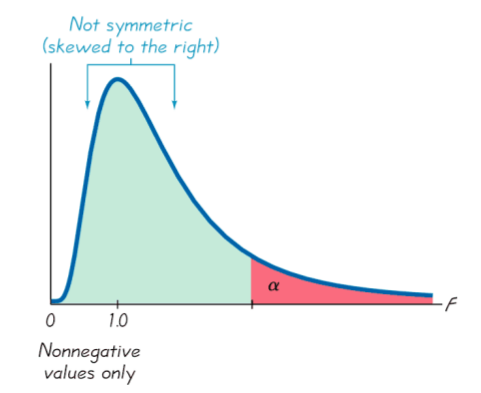
\includegraphics[scale=.2]{images/F.png}
\end{column}

\begin{column}{.7\textwidth}
\footnotesize{
\[
F = \frac{Variância entre fatores}{Variância dentro de cada fator}
\]

\vspace{.5cm}

Assim, se o $F_{calculado}$ cair dentro da área $\alpha$ de
``Rejeição'', temos evidências suficientes para refutar a $H_{0}$ em
favorecimento da $H_{1}$.

\vspace{.5cm}

Caso contrário, não temos evidências suficientes e falhamos em rejeitar
a $H_{0}$.
}
\end{column}
\end{columns}
\end{block}
\end{frame}

\end{document}


%%%%%%%%%%%%%%%%%%%%%%%%%%%%%%%%%%%%%%%%%%%%%%%%%%%%%%%%%%%%%%%%%%%%%%%%
%% 
%% The MIT License (MIT)
%% 
%% Copyright (c) 2014 Rodrigo Sant'Ana
%% 
%% Permission is hereby granted, free of charge, to any person 
%% obtaining a copy of this software and associated documentation 
%% files (the 'Software'), to deal in the Software without 
%% restriction, including without limitation the rights to use, 
%% copy, modify, merge, publish, distribute, sublicense, and/or 
%% sell copies of the Software, and to permit persons to whom the 
%% Software is furnished to do so, subject to the following 
%% conditions: 
%% 
%% The above copyright notice and this permission notice shall be 
%% included in all copies or substantial portions of the Software.
%% 
%% THE SOFTWARE IS PROVIDED 'AS IS', WITHOUT WARRANTY OF ANY KIND, 
%% EXPRESS OR IMPLIED, INCLUDING BUT NOT LIMITED TO THE WARRANTIES 
%% OF MERCHANTABILITY, FITNESS FOR A PARTICULAR PURPOSE AND
%% NONINFRINGEMENT. IN NO EVENT SHALL THE AUTHORS OR COPYRIGHT HOLDERS 
%% BE LIABLE FOR ANY CLAIM, DAMAGES OR OTHER LIABILITY, WHETHER IN AN 
%% ACTION OF CONTRACT, TORT OR OTHERWISE, ARISING FROM, OUT OF OR IN 
%% CONNECTION WITH THE SOFTWARE OR THE USE OR OTHER DEALINGS IN THE 
%% SOFTWARE.
%% 
%%%%%%%%%%%%%%%%%%%%%%%%%%%%%%%%%%%%%%%%%%%%%%%%%%%%%%%%%%%%%%%%%%%%%%%%
